%`preamble' precedes the main text
\documentclass[12pt, a4paper]{article}

%some important packages
\usepackage[T1]{fontenc}					%package to set font encoding
\usepackage[latin1]{inputenc}				%package to set input encoding
\usepackage[section]{placeins}

%\usepackage[ngerman]{babel} 				%option for paper in german
\usepackage{graphicx} 						%package to include graphics
\usepackage{setspace} 						%package to set space between lines
\usepackage{lscape} 							%package to rotate pages
\usepackage{lipsum} 							%package for random text, delete \lipsum[1]-command when you write your own text
\usepackage{booktabs} 						%package for nice tables
\usepackage{amsmath,amsfonts,amssymb} 	%packages for LaTeX that provides various features to facilitate writing math 									
												%formulas and to improve the typographical quality of their output 
\usepackage{array}							%package for extending array and tabular environments
\usepackage{textcomp}						%package support of the text companion fonts
\usepackage{exscale} 							%package for nice summation sign 
\usepackage{tabularx} 						%package for column width and linebreaks in table cells
\usepackage{natbib}							%package for bibliography
\usepackage{ragged2e} 						%package provides less extreme raggedness than the standard LaTeX commands \flushleft and \flushright
\usepackage{multirow}           					%package to combine cells in tables
\usepackage{eurosym} 						%package to get eurosymbol per \euro
\usepackage{verbatim}						% package for verbatim evironment
\usepackage{float}						%package to define position of tables and figures
\usepackage{color}
%adjustment of page parameters
\usepackage[left=3cm, right=2cm, top=2.5cm, bottom=2.5cm]{geometry}
\renewcommand{\baselinestretch}{1.5} 		%line spacing is set to 1.5
\setlength{\footnotesep}{10.0pt}				%space between footnote and text


%title
\title{{\Large Do voting systems affect segregation\footnote{This paper was written as a term paper in the course XYZ at the Chair of Economics VI: Empirical Economics, Prof. Dr. Mario Larch, University of Bayreuth.}}\\
\vspace{3mm}{\Large Term Paper, Software Engineering for Economists}%options: BA Thesis, MA Thesis etc.
}

%author
\author{Julia Baumann\footnote{4th semester, BA Economics. Student No.: 2323235. Address: Joseph-Schumpeter-Allee 42, 95444 Bayreuth. Tel.: +31 415 926 535 897. Email: market.frictions@uni-bayreuth.de.}\\ Tadas Gedminas\\Axel Purwin}
\date{Autumn 2017}
%beginning of the main text
\begin{document}

\maketitle \thispagestyle{empty}

%abstract
\begin{abstract}

%temporary set single space
\setlength{\baselineskip}{10.5pt} 

\vspace{0.5cm} 
\noindent You should put your abstract here. 
\vspace{0.5cm} 

{\normalsize \noindent \emph{JEL-Codes}:  Code1, Code2, Code3.\\ % for more information on JEL codes, consult: http://www.aeaweb.org/jel/jel_class_system.php
\emph{Keywords}: Keyword1, Keyword2, Keyword3.} % put some keywords that describe your work here
\end{abstract}

\newpage

%you can comment the following three lines if you write a term paper
\thispagestyle{empty}
\tableofcontents
\newpage

\newpage
\thispagestyle{empty}
\listoftables


\newpage
\thispagestyle{empty}
\listoffigures


\newpage


\setcounter{page}{1}%set page number to one

%*******************************************************************************************************************************************************************
%*******************************************************************************************************************************************************************
%*******************************************************************************************************************************************************************
%*******************************************************************************************************************************************************************
%main content

\section{\label{sec_intro}Introduction}

In 1969 Thomas Schelling published his influential article "Models of Segregation" in \textit{The American Economic Review}. In the article Schelling uses an agent-based model to show that although \textit{individuals} might have high tolerance towards other races the aggregated outcome will still be clear ethnic segregation. Ethnicity is, of course, not the only segregating factor in societies. In the book "The Big Sort" (2008), the journalist Bill Bishop and the sociologist and statistician Robert Cushing argue that Americans now increasingly segregate themselves also along political affiliations. In their arguing, Bishop and Cushing point to the fact that the number of counties that was won by a landslide by either the Republicans or the Democrats has increased dramatically since the 1970s. 
\newline In this short paper we will use an agent-based model similar to Schelling's to find out whether the magnitude of political segregation depends is affected by the type of voting system in a country. More specifically we will simulate political segregation using three different election models: first-past-the-post with two parties (e.g. USA), first-past-the-post with several parties (e.g. UK) and instant-runoff voting (e.g. Australia). This brief paper begins with a literature review, in which we highlight papers that discuss segregation, or geographical sorting, based on political opinions. We then explain our agent-based model and how it slightly varies depending on the election system imposed. Finally, we report and discuss our results.


%*******************************************************************************************************************************************************************
%*******************************************************************************************************************************************************************
\section{Literature Review}\label{lit}
There is a plethora of articles that look into the reasons as to why people move and how these individual decisions combine to form larger migration patterns. The number of papers that explicitly investigate the extent to which people move and live according to political convictions is, however, considerably smaller. Nonetheless, there are several papers that deal with this issue in an American context and a couple of papers that use British data. 
\newline Buscha et al. (2014) use data from the British Household Panel Survey to track individuals' political preferences and place of residence over a eighteen-year period. They use the panel data set to regress political preferences on the type of move undertaken in the last five years (from a labour constituency to a conservative constituency, from a liberal constituency to a labour constituency etc.) as a well as a number of control variables (e.g. sex, age, income). Their findings suggest that there is both a "political assimilation effect" (p. 546) (i.e. that people tend to adapt their political views to the majority views of the constituency they are moving in to) and a selection into areas (i.e. people with a certain political opinion tend to move into areas where the majority shares this opinion). This self selection effect does, however, disappear almost completely when the authors control for individual socio-economics characteristics, leading them to draw the conclusion that the political segregation is mainly a consequence of the fact that people who share socio-economic background also tend to share  political conviction.   
\newline Tam Cho, Gimpel and Hui (2012) track migration flows (i.e. moving from one ZIP code to another within the state or moving to an adjacent state) in seven US states between 2004 and 2008. They use hierarchical linear models, regressing change in partisan spread (i.e. the difference between Republican and Democrat voting registration rates) between the district the individual is moving from and the district the individual is moving to on a number of variables, including age, party affiliation and median income change. Like Buscha et al., Tam Cho et al. find that it is the economic factors that are most decisive when people decide where to move. They do, however, also find evidence that point to partisan composition of the moving destination being a factor in people's choice of new homes. 
\newline In his article "Migration and Sorting in the American Electorate: Evidence from the 2006 Cooperative Congressional Election Study" (2011) Ian McDonald matches election survey data with the US Postal Service's change-of-address database to examine whether an individual's ideological preference predicts the individual's moving destination (defined as congressional district). McDonald estimates a logit regression with the migrant's destination district partisanship as dependent variable and ideology and the political majority in the origin district, as well as covariates, as independent variables. McDonald finds that the migrant's new home district is more likely to be an ideological match than the district which the migrant left, indicating that Americans do indeed take the political views of their future neighbours into consideration when moving. 

%*******************************************************************************************************************************************************************
%*******************************************************************************************************************************************************************
\section{\label{model}The Election Models}
To answer the question how different voting systems influence the degree of political segregation in a country, we employ an agent-based model. Our hypothesis is that voting systems introduce different degrees of political representation, which will affect the probability with which agents will move. In this section, we present the general setup of our model as well as the individual electoral systems that we will simulate in the subsequent analysis.\\%necessary here? - should be in the intro I think\footnote{An agent-based model is, in short, a model where you simulate the actions of autonomous individual agents and evaluate the effects that these individual actions have on the system as a whole.}.
Note that all model societies are comprised of four types that correspond to different preferences on the political spectrum.\footnote{This is for reasons of comparability between societies. We set The proportion of types to 33\% for the types on the edges of the political spectrum and to 17\% for each of the two moderate types.} Agents obtain utility from having neighbors that are exactly their type but can also gain some utility from people that have voted for the same party (as their first-order preference) but are a different type. In addition to benefiting from having similar neighbors, agents also gain when their party has won the local elections. How much weight they put on the election outcome will be varied in the simulation.
Thus, we construct the individuals' utility function such that it consists of the utility derived from the number of like-minded neighbors and the utility derived from living in a county that is ruled by the party they favor.
We impose a threshold utility that specifies the units of utility an agent must have to be happy. If the agent's utility is below this threshold the agent will move (and thus leave their house vacant), randomly, into a house until they find a place that gives them a utility that is above the threshold level. Initially, agents are randomly assigned to houses in the different local areas. We set 30\% of houses to be empty to leave some space for individuals to move.
 In our simulations, our society consists of $33\times33$ -houses square. Each county is $11\times11$ houses (our society thus consists of nine counties) and each neighborhood is $3\times3$ houses, where the agent whose neighborhood it is naturally lives in the middle of this $3\times3$ matrix. (In our model we also let northern and southern, and eastern and western, borders of the square meet, so that the agents living on the edge of the square are also completely surrounded by houses, and thus living in neighborhoods.)
%We then run the simulations until all agents have found a house in which their utility is above the threshold value. % Not exactly right

\subsection{USA: First-past-the-post with two parties}
For the US model society, one can think of the four types of agents as republicans, moderate republicans, democrats and moderate democrats. The society is then divided into smaller local areas, counties 
%not states?
, such that each individual lives in a county that is either republican or democrat depending on the majority view in the county. Our individuals, 33\% republicans and democrats respectively and 17\% moderate republicans and moderate democrats, respectively. %, are initially randomly assigned to the houses in the different counties. A set \textcolor{red}{20} per cent of the houses are also empty, such that the individuals can move.
Thus, in the whole society there will be 50\% of agents voting for each party. Of course, this distribution can vary quite significantly across counties, so that it is a priori not clear, whether a county will be blue or red.
The electoral system of the US is such that there are two parties\footnote{We abstract away from small parties that exist in the US in reality.} that compete in local elections. The party that gets the majority of votes (here in both absolute and relative terms), wins the county. All types will want to vote for one of the two parties: Republicans and moderate republicans vote for the same party and democrats and moderate republicans together vote for the other party. Agents gain election utility if and only if they live in a county where their political view is held by the majority of the individuals.  Formally, we can write individuals' utility function as follows:


\begin{equation}
U_i=t_{same_i}+\alpha \, t_{similar_i}+\gamma \, election_{win_c}
\end{equation}

where $t_{same}$ is the number of neighbors, i.e. agents in adjacent parts of the grid, that have the same type as the individual. $t_{similar}$ is the number of neighbors that voted for the same party but are not the same type. For example, a republican type derives some utility from living next to a moderate republican but possibly not as much as from living to someone who is also a pure republican. We set $\alpha$ to varying values in the analysis. Lastly, $election_{win}$ is an indicator variable that takes on the value 1 if the individual's preferred party won the county election. When $U_i < \bar{U}$, the agent will relocate to a new location.

\subsection{UK: First-past-the-post with several parties}
In this model we add a third party to our society, so that agents have the option to vote for either Left, Right, or Center. The four agents therefore now split their votes between the three parties such that the two more moderate types in the middle both vote for the center party. This implies that the center party has a left and a right wing, whereas the two parties on the edges are more homogeneous in the sense that only one type will want to vote for them. We maintain the same distribution of types as in the case of the US elections, i.e. 33\% right-wing, 17\% center-right, 17\% center-left, and 33\% left. Therefore, 33\% of the individuals in the model society vote for the right party, 33\% vote for the left party, and in total 34\% vote for the center party. \\
While this may accurately reflect the real-world situation of political types in the UK, we would like to capture a feature of this electoral system: Compared to the US, elections in the UK usually feature more than two parties that obtain a significant share of votes. At the same time, they maintain the first-past-the-post principle, which implies that a party in the UK only has to obtain the relative majority of votes, and not necessarily an absolute majority. From this follows that, compared to the US, less agents tend to find themselves represented by the party they voted for in the elections.\footnote{This of course requires that the party landscape reflects the real preferences of citizens. One may doubt that this is always the case in reality. However, since we only look at fully developed democracies, we assume that parties exist according to the real preferences of people.} For instance, a party could win with 34\% of votes when the other two parties each obtained 33\% of votes each. This means that only 34\% of agents in this county would get utility from the election outcome while 66\% have no utility from this political situation. In the US, the maximum that does not feel represented will always be at most 50\%. It may therefore be more likely that agents in the UK model move, because overall less individuals will get the election utility which will therefore make it more difficult to reach the threshold utility for being happy.
The utility function for the individual in the UK model society is the same as in equation (1).


\subsection{Australia: Instant run-off voting} 
In our society with instant run-off voting, first-order preferences are the same as in the UK model: Four types vote for three different parties, where the two moderate types vote for the center. The distribution of types is the same as in the other simulations. \\
The difference is that we now have a different election rule where second-order preferences matter: If no party gains the absolute majority in the first round, the second preference of the agents who voted for the party with the least votes is taken into account and these votes are added to the two other parties. Let us consider an example where the election outcome is such that no party reaches absolute majority and the center party gained the least votes. In this case, the center party voters, who have submitted their second-order preferences along with their first preference, are revisited: Moderate right-wing agents now vote for the right party and moderate left-wingers submit their vote for the left party. Their votes are added to the number of votes the left and right party had obtained in the first round. Since one party has been eliminated, there are only two parties left now and one must obtain at least 50\% of votes in the second round. This principle is applied no matter what party initially gained the least votes: If the right party or center party are the least popular, their voters will prefer the center party as their second vote. \\
We assume that agents whose second-order preference was counted in the election get a lower utility from the outcome if that second rank won than when their first ranked preference wins. This is reflected in a utility function that is now slightly different than in the other societies: % A bit too complicated

\begin{equation}
U_i=t_{same_i}+\alpha \, t_{similar_i}+\gamma \, election_{1win_c} + 0.5 \, \gamma \, election_{2win_c}
\end{equation}

where $t_{same}$ and $t_{similar}$ are defined as before. Agents get utility $\gamma$ if their top preferred party wins the election and $0.5 \gamma$ if their favorite party gains the least votes in the first round but their second-order preference wins the election overall.
The Australian system implies that compared to the UK system, more agents should feel somewhat represented by the electoral outcome: Since they get to submit a list of preferences such that they can still influence their local election if they like the least popular party most, it is more likely that they will gain at least some utility from the outcome.
 %Each of our four different agents then ranks its preferences in the election. The two agent types on the extremes (farthest to the right or farthest to the left on the political axis) naturally rank their political choices accordingly. The two types in the middle, leaning either right or left, rank the extreme type of their political camp as their second choice. If any party gets more than 50 per cent of the top rank votes this party wins, if not, the party with the smallest amount of top rank votes is elimaned and the second rank votes from these ballots are counted to the election. This procedure continues until a party gets more than 50 per cent of the votes. \textcolor{red}{If the voting count is 50-50...}

%*******************************************************************************************************************************************************************
%*******************************************************************************************************************************************************************


%*******************************************************************************************************************************************************************
%*******************************************************************************************************************************************************************



%*******************************************************************************************************************************************************************
%*******************************************************************************************************************************************************************

\section{\label{sec_res}Analysis}
We run the model 100 times. Each time the model runs 100 steps (obviously, the iterations will stop, should all agents have found a neighborhood in which they are satisfied). The mean values of each step for each different model are shown in figures 1 through 8. In total we run the model 7 times, that is, we use 7 different combinations of parameter values. Our baseline model uses the middle values for the parameters, i.e. the weight of living with like-minded neighbors is set to 0.5, the weight on election is set to 1 and the threshold utility is set to 5. In the other 6 runs we vary one parameter value at the time, either up or down, while keeping the remaining two parameter values at the baseline, "middle", level % T: to be consistent, a single run simulates the model 100 runs, and for each setup with different parameters we run the models 100 times
. The different parameter values are shown in Table 1. We evaluate the model on three measures: "Information Value", "Share of Happy Agents" and "Share of Segregated Agents". The "Information Value" measures how much the counties differ from each other. If all counties have similar shares of the different agent types the "Information Value" is low, if the counties differ alot (and thus are more segregated) the value is high. The formula for the "Information Value" is as follows: \newline \newline
$$\sum_{m=1}^{M}\sum_{j=1}^{J}\frac{t_j}{T \cdot E}\pi_{jm}ln\frac{\pi_{jm}}{\pi_m},$$ where M is the number of agent types, J is the number of counties, T is the total number of agents, E$=\sum_{m=1}^{M}\pi_m ln(\frac{1}{\pi_m})$, i.e. \textcolor{red}{Entropy??}, $\pi_{jm}$ is the proportion of agent type $m$ living in county $j$ and $\pi_m$ is the proportion of agent type $m$. This formula for measuring segregation is used by Reardon and Firebaugh (2002). %T: Include motivation for why information value is preferred aggregate measure of segregation 

\begin{table}[ht]
	\centering
	\caption{Utility model, parameter values}
	\begin{tabular}{llll}
		\hline
		Parameter values & Neighbourhood ($\alpha$) & Election ($\gamma$) & Threshold ($\bar{U}$) \\ 
		\hline \hline
		Low & 0.25 & 0.5 & 4 \\ 
		Middle & 0.5 & 1 & 5 \\ 
		High & 0.75 & 1.5 & 6 \\ \hline
		\hline
	\end{tabular}
\end{table}

Figure 1 shows the three model measurements for the baseline model ( \textcolor{red}{why is "share of happy" different from the middle graph in the three different varying utility parameters graphs??}) %T: when doing different parameter comparisons, the baseline case is re-simulated hence the final graphs are not identical
. It is clear that the society with a first-past-the-post with several parties election system (from here on "UK"), is most segregated. When it comes to the share of happy agents UK and US seem to converge. That the UK is not also the most happy society, in a setting where a certain amount of segregation leads to agent happiness, can be explained by the fact that there are three parties in the UK and the consequently even though the society as a whole is more segragated than in the US, less agents will be represented politically and they will thus derive less utility from the election result. Figure 2 breaks down the segregation generated by the baseline model into the agent groups. Not surprisingly, the UK sees the highest levels of group segregation. Also the American and Australian agent groups show an expected pattern. Naturally, the two political extremes can and will segregate themselves. The center agents in the US cannot live in a county where there party rules and will thus to a larger extent live among agents who do not share their center ideology. In Australia, on the other hand, the center parties can rule, which is why we see that the two center groups are more segregated in Australia than in the US; it will simply be more attractive for a center agent to live with other center agents. \newline \newline
Figures 3 through 8 show the same two graphs for the parameter value variations. The relative relation between the three countries in terms of degree of segregation remains stable for the different parameter values. Figures 4 and 6 supports the aggregate findings that although it is generally less segregated than the US and the UK, Australia sees a relatively higher of segregation among the center groups. When varying the election paramater value from 1 to 1.5 we see that the share of happy agents becomes higher in Australia than in the US (Figure 3). The reason for this can be inferred from Figure 4: the relatively bigger importance of elections means that Australia, where all parties can win elections, will see more movements from the agents, escpecially the center ones, and in the end more segregation, which in our model will lead to a greater share of happy agents. In Figures 5 and 6 we see that the level of segregation is unaffected by changes in the neighbourhood utility parameter value. This makes sense, sinse the utility derived from like-minded neighbours is the same for all three societies. When we vary the threshold utility from 5 to 4 Australia becomes relatively (and absolutely) more segregated. This is due to the same mechanism that led to more segregation when the importance of elections increased, namely that when the agents move more easily the probability that the Australian center agents will find their likes and creating an election winning firmly segregated county increases. The effect of more easily moving agents is smaller for the US and the UK since they have fewer parties. In Figure 8 we can see that the increasing segregation in Australia is indeed driven by the increasingly segregated center agents.        

\begin{figure}[bp!]
	\centering
	\caption{Aggregate Ratios}
	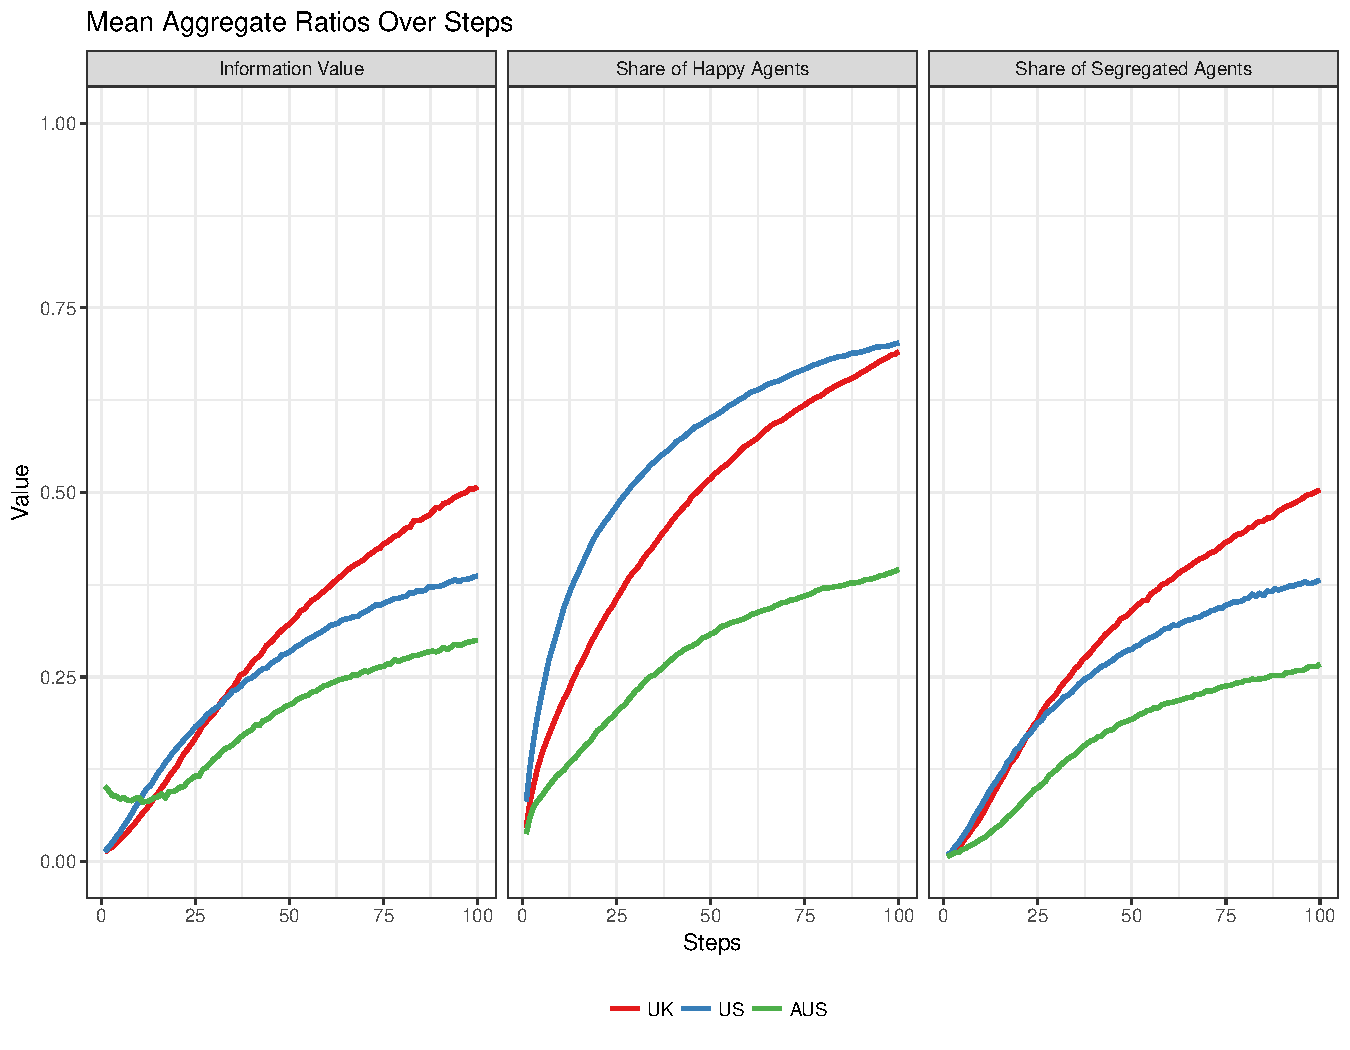
\includegraphics[scale=0.6]{./Plots/agg_ratios.pdf}
\end{figure}

\begin{figure}[bp!]
	\centering
	\caption{Group Segregation}
	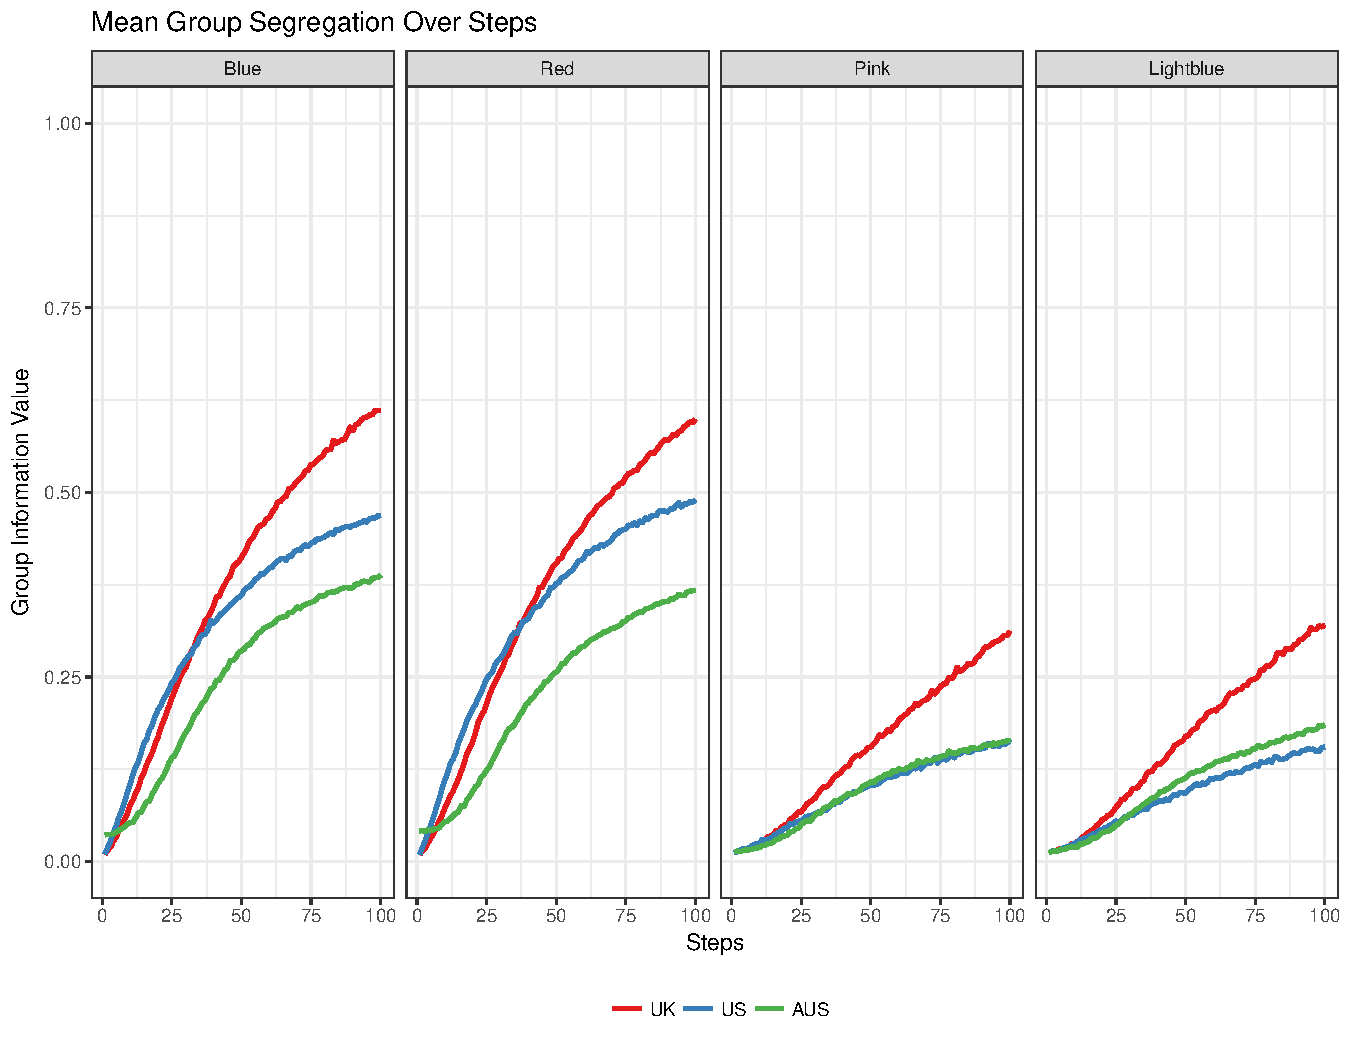
\includegraphics[scale=0.6]{./Plots/grp_ratios.pdf}
\end{figure}

\begin{figure}[bp!]
	\centering
	\caption{Aggregate Ratios and Election Utility}
	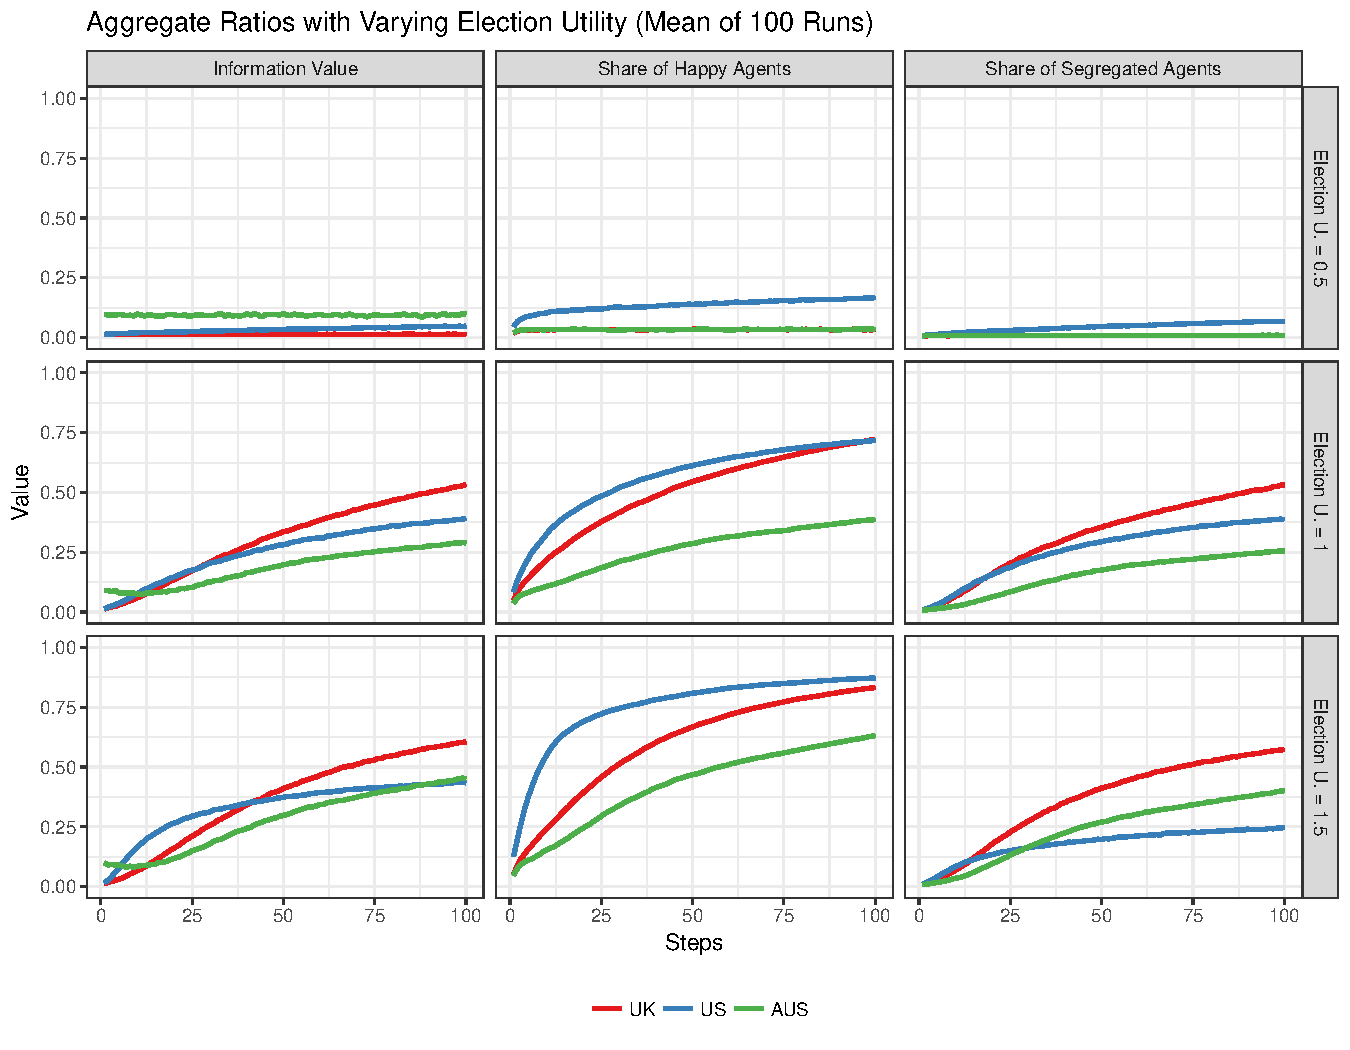
\includegraphics[scale=0.6]{./Plots/el_agg_ratios.pdf}
\end{figure}

\begin{figure}[bp!]
	\centering
	\caption{Group Segregation and Election Utility}
	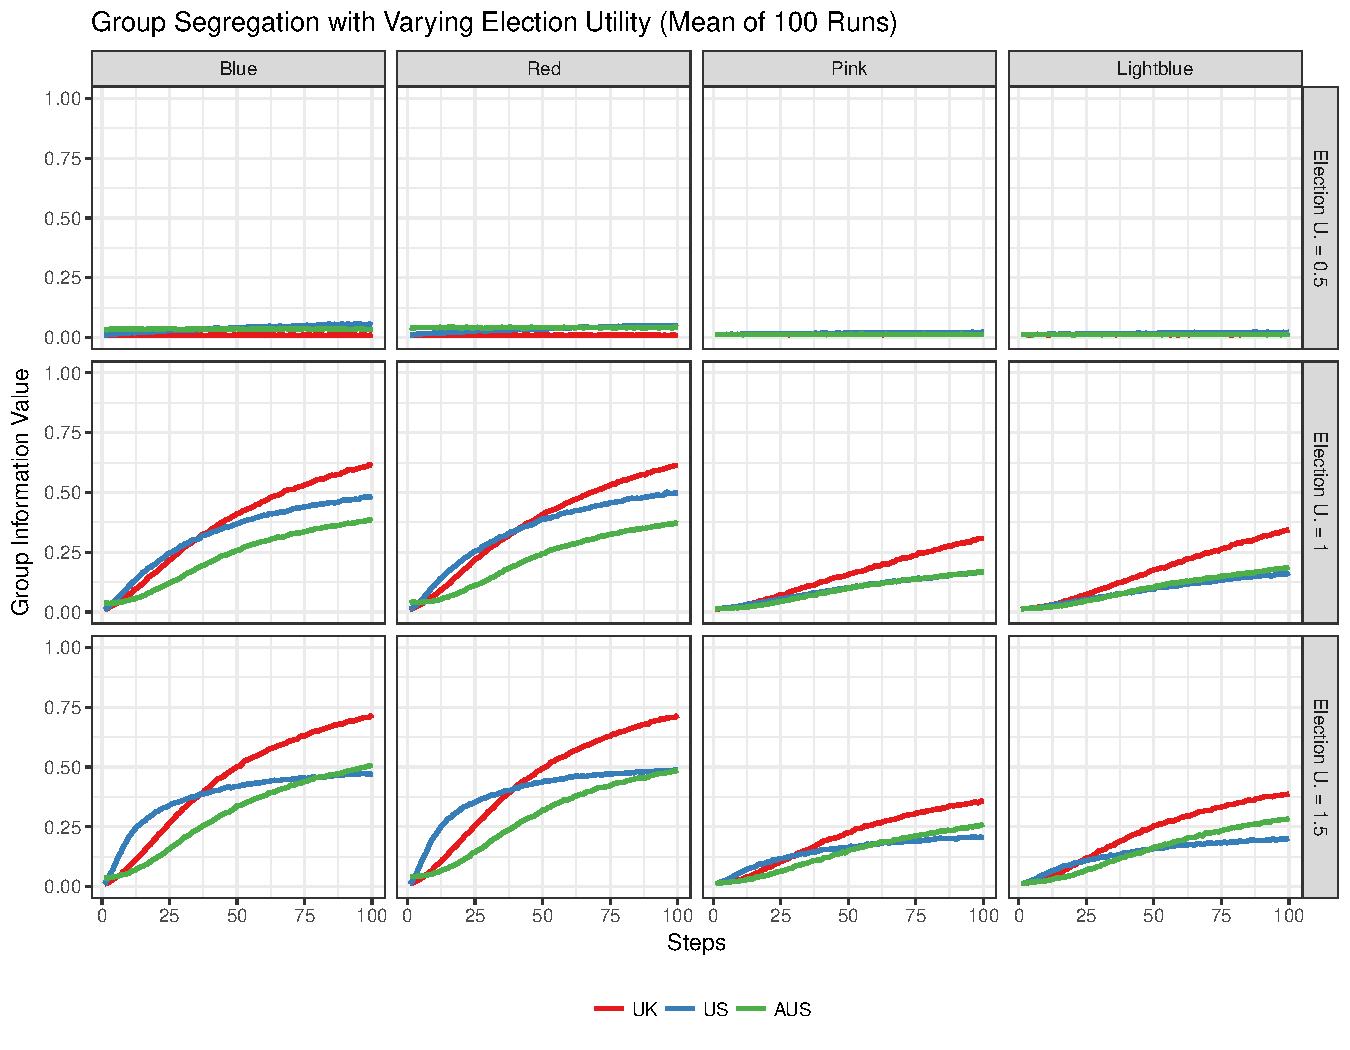
\includegraphics[scale=0.6]{./Plots/el_grp_ratios.pdf}
\end{figure}

\begin{figure}[bp!]
	\centering
	\caption{Aggregate Ratios and Neighbourhood Utility}
	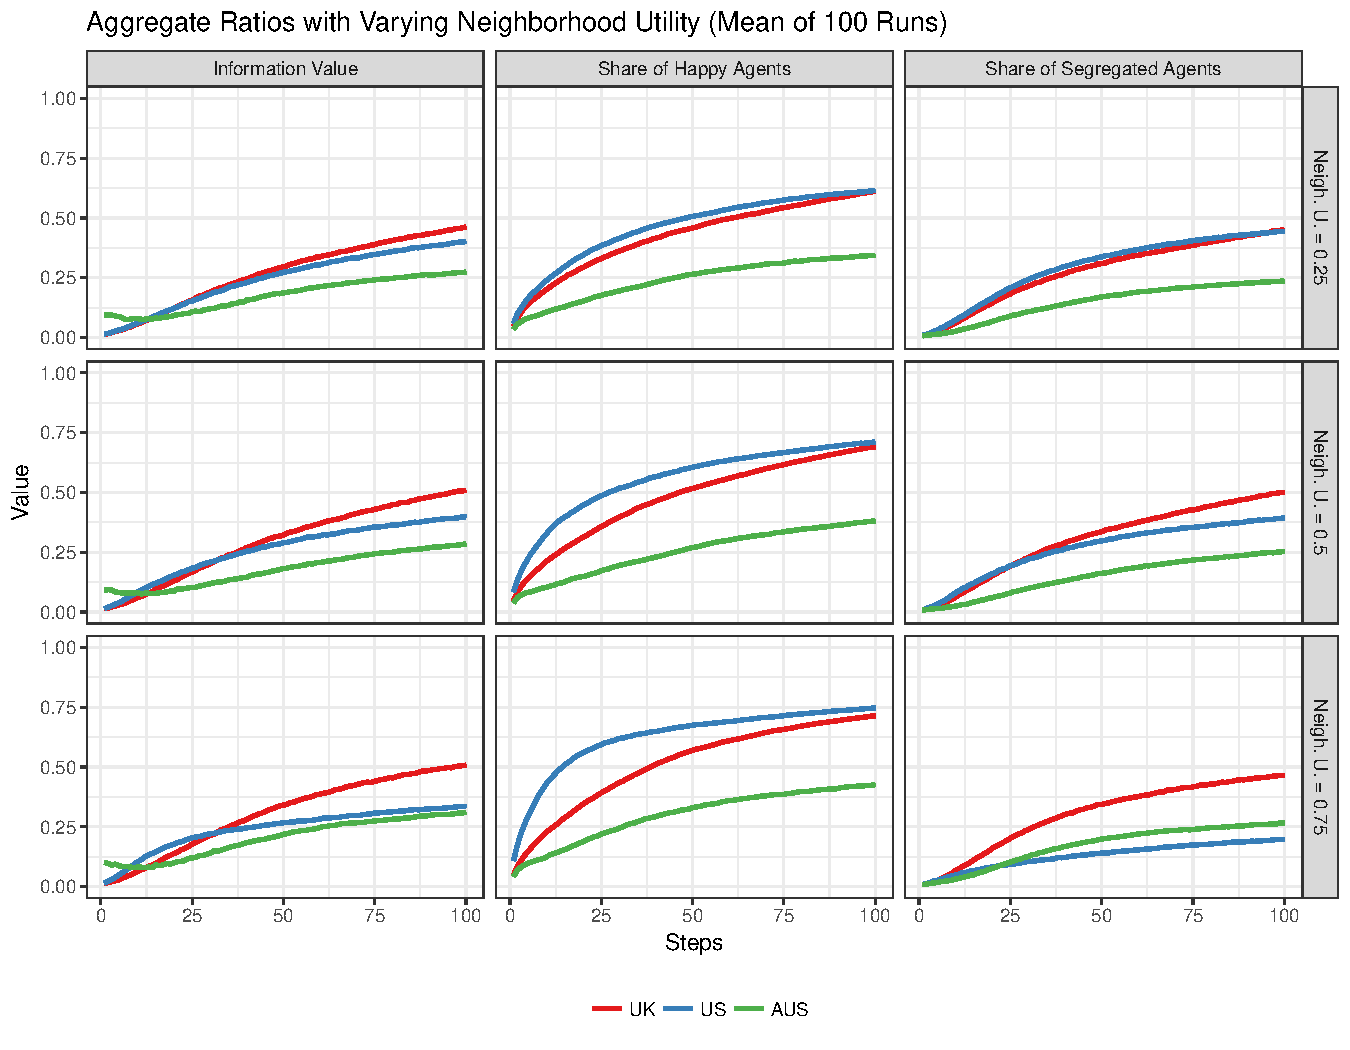
\includegraphics[scale=0.6]{./Plots/nb_agg_ratios.pdf}
\end{figure}

\begin{figure}[bp!]
	\centering
	\caption{Group Segregation and Neighbourhood Utility}
	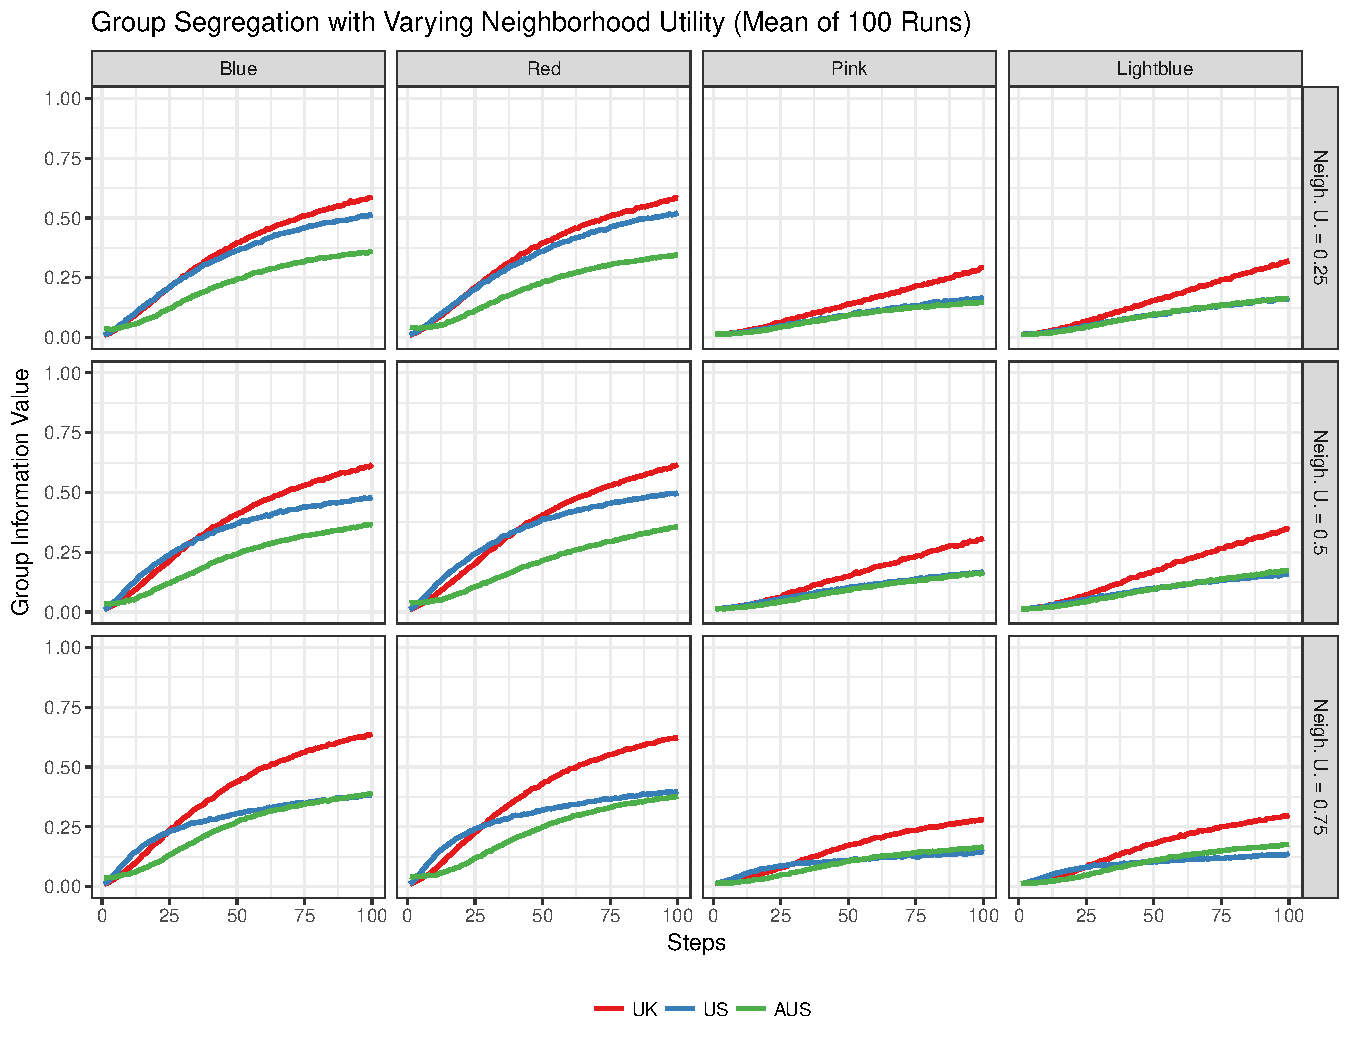
\includegraphics[scale=0.6]{./Plots/nb_grp_ratios.pdf}
\end{figure}

\begin{figure}[bp!]
	\centering
	\caption{Aggregate Ratios and Threshold Utility}
	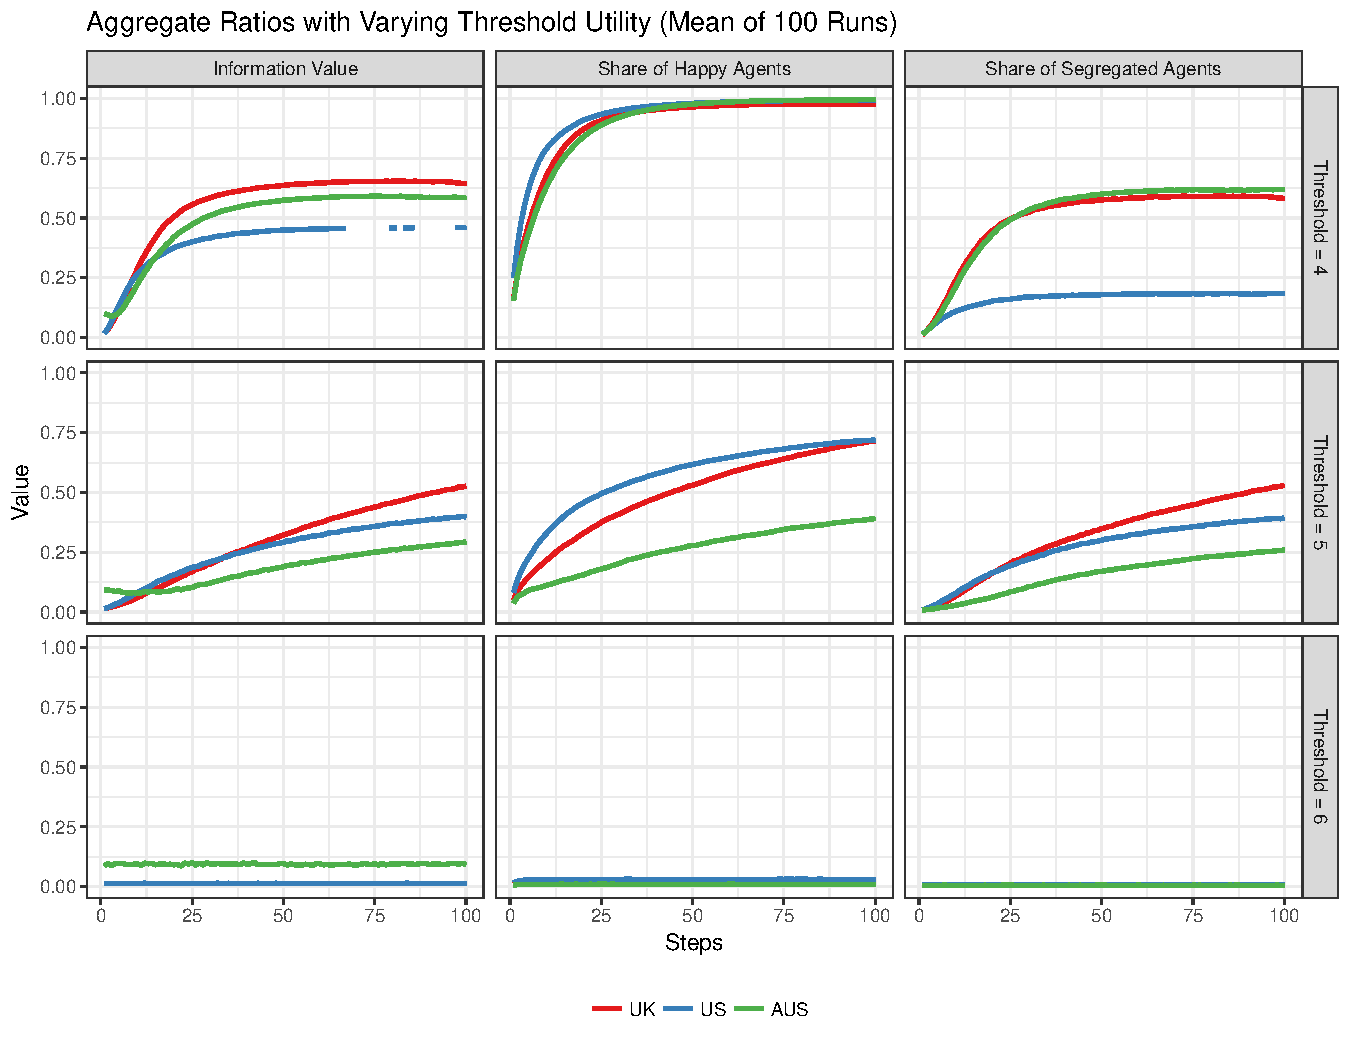
\includegraphics[scale=0.6]{./Plots/th_agg_ratios.pdf}
\end{figure}

\begin{figure}[bp!]
	\centering
	\caption{Group Segregation and Threshold Utility}
	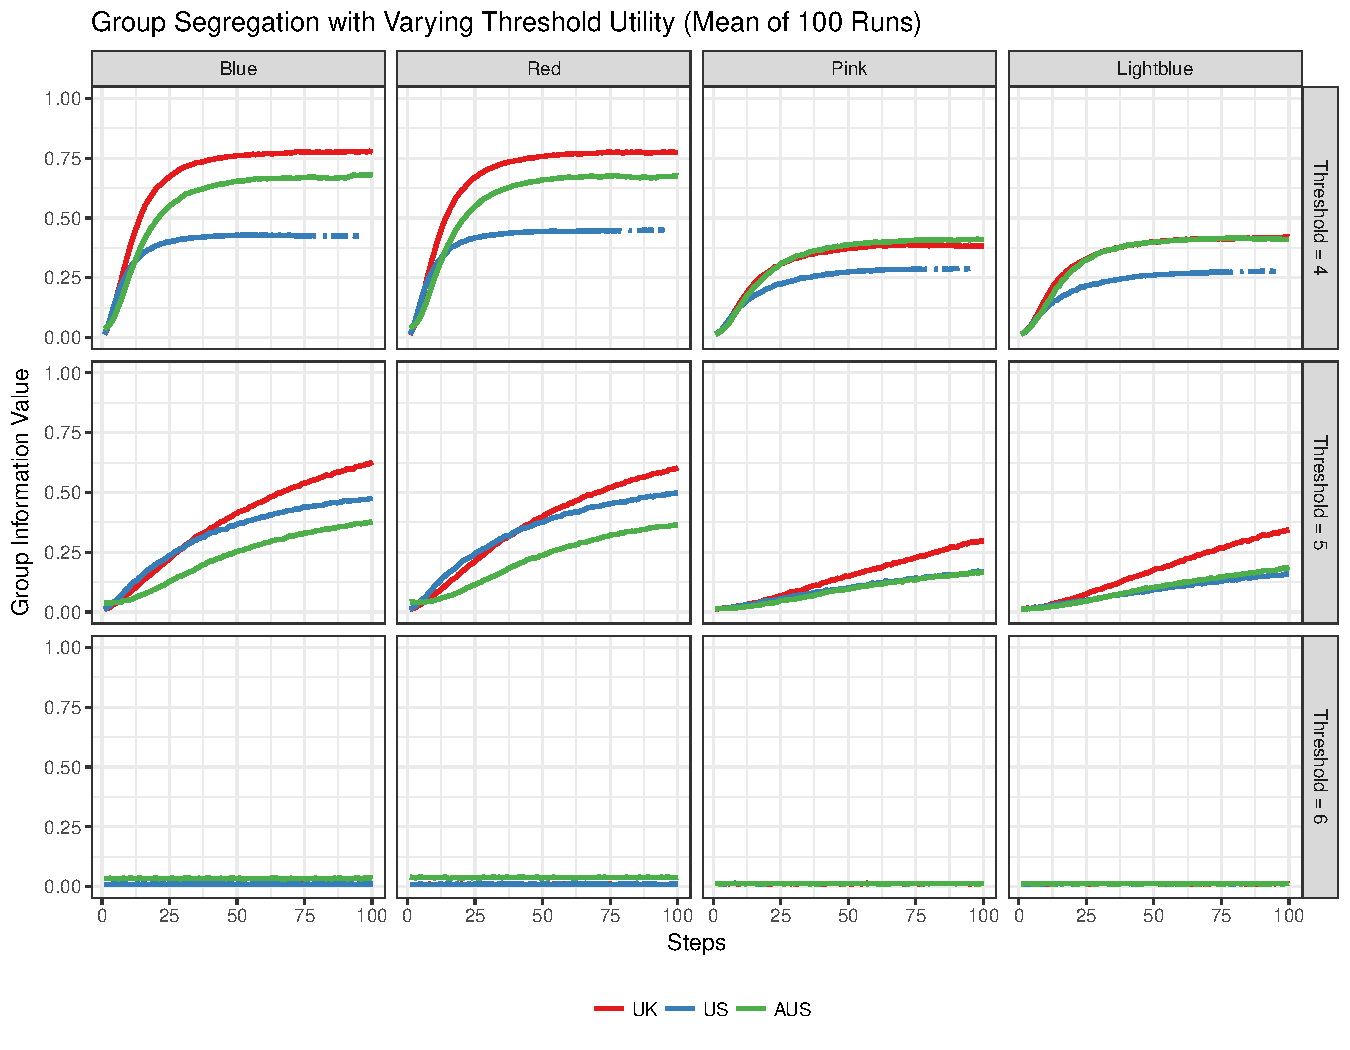
\includegraphics[scale=0.6]{./Plots/th_grp_ratios.pdf}
\end{figure}


%*******************************************************************************************************************************************************************
%*******************************************************************************************************************************************************************

\section{\label{sec_conc}Conclusion}


%*******************************************************************************************************************************************************************
%*******************************************************************************************************************************************************************

%reference section with econometrica style. there are two options. the first is to use a bibtex-file. this can be very helpful in a paper with many reference. the second is to write down the referenes by hand. 

\newpage

%Version 1
%\bibliographystyle{econometrica}
%\bibliography{bibliography}

%Version 2
\section*{\label{sec_ref}References}

BUSCH ET AL. (2014):`` Places and Preferences: A Longitudinal Analysis of Self-Selection and Contextual Effects,'' \textit{British Journal of Political Science} 46, 529-550.

\noindent MCDONALD, I. (2011):`` Migration and Sorting in the American Electorate: Evidence From the 2006 Cooperative Congressional Election Study,'' \textit{American Politics Research} 39(3), 512-533.

\noindent TAM CHO, W. K., GIMPEL, J. G. AND HUI, I. S (2012): ``Voter Migration and the Geographic Sorting of the
American Electorate,'' \textit{Annals of the Association of American Geographers}, DOI:10.1080/00045608.2012.720229.

\noindent REARDON, S. F. and FIREBAUGH, G. (2002):``Measures of Multigroup Segregation," \textit{Sociological Methodology} 32: 33-67, DOI: 10.1111/1467-9531.00110. 




\end{document}
%the  end 